
\documentclass{beamer}
\usecolortheme{dove}
\setbeamertemplate{navigation symbols}{}
\usepackage{amsmath,amssymb,amsfonts,amsthm, multicol, subfigure, color}
\usepackage{bm}
\usepackage{graphicx}
\usepackage{tabularx}
\usepackage{booktabs}
\usepackage{hyperref}
\usepackage{pdfpages}
\usepackage{xcolor}
\definecolor{seagreen}{RGB}{46, 139, 87}
\def\independenT#1#2{\mathrel{\rlap{$#1#2$}\mkern2mu{#1#2}}}
\newcommand\indep{\protect\mathpalette{\protect\independenT}{\perp}}
\def\log{\text{log}}
\newcommand\logit{\text{logit}}
\newcommand\iid{\stackrel{\text{iid}}{\sim}}
\newcommand\E{\text{E}}
\newcommand\V{\text{V}}
\renewcommand\P{\text{P}}
\newcommand{\Cov}{\text{Cov}}
\newcommand{\Cor}{\text{Cor}}
\newcommand\doop{\texttt{do}}
\usepackage{stackrel}
\usepackage{tikz}
\usetikzlibrary{arrows,shapes.arrows,positioning,shapes,patterns,calc}
\newcommand\slideref[1]{\vskip .1cm \tiny \textcolor{gray}{{#1}}}
\newcommand\red[1]{\color{red}#1}
\newcommand\blue[1]{\color{blue}#1}
\newcommand\gray[1]{\color{gray}#1}
\newcommand\seagreen[1]{\color{seagreen}#1}
\newcommand\purple[1]{\color{purple}#1}
\newcommand\orange[1]{\color{orange}#1}
\newcommand\black[1]{\color{black}#1}
\newcommand\white[1]{\color{white}#1}
\newcommand\teal[1]{\color{teal}#1}
\newcommand\magenta[1]{\color{magenta}#1}
\newcommand\Fuchsia[1]{\color{Fuchsia}#1}
\newcommand\BlueGreen[1]{\color{BlueGreen}#1}
\newcommand\bblue[1]{\textcolor{blue}{\textbf{#1}}}
\newcommand\bred[1]{\textcolor{red}{\textbf{#1}}}
\newcommand\bgray[1]{\textcolor{gray}{\textbf{#1}}}
\newcommand\bgreen[1]{\textcolor{seagreen}{\textbf{#1}}}
\newcommand\bref[2]{\href{#1}{\color{blue}{#2}}}
\colorlet{lightgray}{gray!40}
\pgfdeclarelayer{bg}    % declare background layer for tikz
\pgfsetlayers{bg,main} % order layers for tikz
\newcommand\mycite[1]{\begin{scriptsize}\textcolor{darkgray}{(#1)}\end{scriptsize}}
\newcommand{\tcframe}{\frame{
%\small{
\only<1|handout:0>{\tableofcontents}
\only<2|handout:1>{\tableofcontents[currentsubsection]}}
%}
}

\usepackage[round]{natbib}
\bibliographystyle{humannat-mod}
\setbeamertemplate{enumerate items}[default]
\usepackage{mathtools}
\usepackage{ulem}

% Need to add examples

\newcommand{\goalsframe}{\begin{frame}{Learning goals for today}
At the end of class, you will be able to:
\begin{enumerate}
\item Define principal strata
\item Understand how they address a post-treatment problem
\item Make assumptions to draw inference about a latent stratum
\end{enumerate} \vskip .2in
\end{frame}}

\title{20. Principal Stratification (Part 1)}
\author{Ian Lundberg\\Cornell Info 6751: Causal Inference in Observational Settings\\Fall 2022}
\date{2 Nov 2022}

\begin{document}

\maketitle

\goalsframe

\begin{frame}{A hypothetical setting}

\begin{itemize}
\item Suppose you have a new exercise program \hfill $A = 1$ vs $A = 0$ \pause
\item You study the effect on heart rate after 12 months \hfill $Y^1 - Y^0$ \pause
\item But only some of the people survive \hfill $M = 1$ \pause
\begin{itemize}
\item And survival was higher in your program
\end{itemize} \pause
\end{itemize} \vskip .1in
\begin{center}
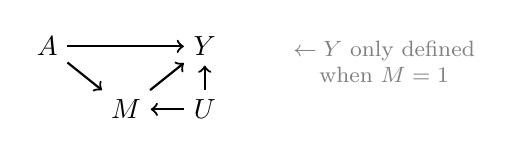
\begin{tikzpicture}
\node (a) at (0,0) {$A$};
\node (m) at (1,-.8) {$M$};
\node (y) at (2,0) {$Y$};
\node (u) at (2,-.8) {$U$};
\draw[->, thick] (a) -- (m);
\draw[->, thick] (a) -- (y);
\draw[->, thick] (m) -- (y);
\draw[->, thick] (u) -- (m);
\draw[->, thick] (u) -- (y);
\node[anchor = west, font = \footnotesize, gray, align = center] at (3,-.2) {$\leftarrow Y$ only defined\\when $M = 1$};
\end{tikzpicture}
\end{center}
How would you analyze this?
\end{frame}


\begin{frame}{A hypothetical setting: Common solutions}
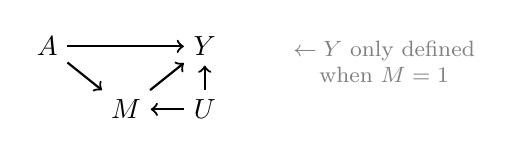
\begin{tikzpicture}
\node (a) at (0,0) {$A$};
\node (m) at (1,-.8) {$M$};
\node (y) at (2,0) {$Y$};
\node (u) at (2,-.8) {$U$};
\draw[->, thick] (a) -- (m);
\draw[->, thick] (a) -- (y);
\draw[->, thick] (m) -- (y);
\draw[->, thick] (u) -- (m);
\draw[->, thick] (u) -- (y);
\node[anchor = west, font = \footnotesize, gray, align = center] at (3,-.2) {$\leftarrow Y$ only defined\\when $M = 1$};
\end{tikzpicture} \pause
\begin{enumerate}
\item Surrogate outcome: Focus on death instead \pause
\item Redefined outcome: Heart rate of dead people is 0 \pause
\item Restrict to those who survived \pause
\begin{itemize}
\item But collider bias: survival is a collider \pause
\end{itemize}
\item Examine the CDE $Y^{11} - Y^{01}$: Force people to stay alive \pause
\begin{itemize}
\item But the mediator intervention is hard to imagine \pause
\end{itemize}
\item New approach: \bblue{Principal stratification}
\end{enumerate}

\end{frame}

\begin{frame}{Principal stratification: The big idea}
Survival $M$ is a \bgray{post-treatment} variable. \vskip .1in
But before the treatment is assigned, there are 4 types of people: \pause
\begin{enumerate}
\item Would survive regardless of treatment \pause
\begin{itemize}
\item $M_i^1 = M_i^0 = 1$
\end{itemize} \pause
\item Would not survive regardless of treatment \pause
\begin{itemize}
\item $M_i^0 = M_i^0 = 0$
\end{itemize} \pause
\item Would survive if and only if they receive the exercise program \pause
\begin{itemize}
\item $M_i^1 = 1, M_i^0 = 0$
\end{itemize} \pause
\item Would survive if and only if the do not receive the program \pause
\begin{itemize}
\item $M_i^1 = 0, M_i^0 = 1$
\end{itemize}
\end{enumerate}
The effect on $Y$ is only defined for stratum 1.
\end{frame}

\begin{frame}{Principal stratification: The difficulty}
Four principal strata
\begin{enumerate}
\item Would survive regardless of treatment
\item Would not survive regardless of treatment
\item Would survive if and only if they receive the exercise program
\item Would survive if and only if the do not receive the program
\end{enumerate} \vskip .1in \pause
\bblue{Difficulty:} We don't observe the strata. We observe:
\begin{itemize} \pause
\item Survivors in the program\hfill  \pause Mix of 1 and 3  \pause
\item Survivors not in the program \hfill  \pause Mix of 1 and 4 \pause
\item Die in the program \hfill  \pause Mix of 2 and 4 \pause
\item Die without the program \hfill  \pause Mix of 2 and 3
\end{itemize}

\end{frame}

\begin{frame}{Assumption: Monotonicity} \pause

Exercise never hurts people. It only does nothing or helps \pause
\begin{enumerate}
\item Would survive regardless of treatment
\item Would not survive regardless of treatment
\item Would survive if and only if they receive the exercise program
\item \sout{Would survive if and only if the do not receive the program}
\end{enumerate} \vskip .1in \pause
We observe the sets
\begin{itemize}
\item Survivors in the program\hfill   Mix of 1 and 3 
\item Survivors not in the program \hfill   All 1 \sout{Mix of 1 and 4}
\item Die in the program \hfill   All 2 \sout{Mix of 2 and 4}
\item Die without the program \hfill   Mix of 2 and 3
\end{itemize} \vskip .1in \pause
What to do with the sets that are still mixed? \pause \bblue{Bounds}

\end{frame}

\begin{frame}{Principal Stratification: Exercise}

You will learn more by doing bounds yourself! \vskip .1in
The rest of class will be a pen-and-paper \bref{https://github.com/ilundberg/teaching/tree/master/info_6751_causal/class_exercises}{exercise}

\end{frame}

\goalsframe



\begin{frame}{References}

Original paper
\begin{itemize}
\item Frangakis, C. E., \& Rubin, D. B. (2002). \bref{https://onlinelibrary.wiley.com/doi/abs/10.1111/j.0006-341x.2002.00021.x}{Principal stratification in causal inference.} Biometrics, 58(1), 21-29.
\end{itemize}
Good recent summary (assigned on syllabus)
\begin{itemize}
\item Page, L. C., Feller, A., Grindal, T., Miratrix, L., \& Somers, M. A. (2015). \bref{https://journals.sagepub.com/doi/abs/10.1177/1098214015594419}{Principal stratification: A tool for understanding variation in program effects across endogenous subgroups.} American Journal of Evaluation, 36(4), 514-531.
\end{itemize}
Good resource for bounds
\begin{itemize}
\item Imai, K. (2008). \bref{https://doi.org/10.1016/j.spl.2007.05.015}{Sharp bounds on the causal effects in randomized experiments with ``truncation-by-death''.} Statistics \& Probability Letters, 78(2), 144-149.
\end{itemize}

\end{frame}

\begin{frame}{Let me know what you are thinking}

\begin{huge} \bref{https://tinyurl.com/CausalQuestions}{tinyurl.com/CausalQuestions} \end{huge}
\vskip .7in

Office hours TTh 11am-12pm and at \bref{https://calendly.com/ianlundberg/office-hours}{calendly.com/ianlundberg/office-hours}\\Come say hi!

\end{frame}


\end{document}
